\documentclass[letterpaper,10pt,twoside,onecolumn,openany,draft]{book}
\usepackage[bg=none,layout=true]{dnd}
\usepackage{dndnotes}
\usepackage{wallpaper}
\usepackage[]{subfiles}
\usepackage[]{import}
\usepackage[]{datetime} 
\usepackage{tikz, pgfplots}
\usepackage[]{lipsum}
\setcounter{secnumdepth}{1}

\begin{document}
\frontmatter                           
\begin{titlepage}	    
  \begin{tikzpicture}[remember picture,overlay]
    \node[inner sep=0pt] at (current page.center) {
\includegraphics[width=\paperwidth,height=\paperheight]{Test-Title.png}};
  \end{tikzpicture}~
  \newpage

  \begin{center}


    \large
    \vspace*{\fill}
    This is the preface of my notes
    \\~\\ 
    Something something
    \\~\\
    \vspace*{\fill}

  \end{center}
  \let\thefootnote\relax\footnote{Disclaimer: You can add some cheeky disclaimer just like the real books.}
\end{titlepage}

\tableofcontents

\mainmatter

\twocolumn
\part{Introduction to the dnd package}

\chapter{Sectioning}
\DndDropCapLine{T}{his package is designed to aid you in} 
writing beautifully typeset lecture notes in the style of the fifth edition of the world's greatest role playing game, Dungeons and Dragons.
It starts by adjusting the section formatting from the defaults in \LaTeX{} to something a bit more familiar to the reader. 
The chapter formatting is displayed above. 
The start of a chapter will always be on a new page. 

\section{Section}
Sections break up chapters into large groups of associated text. Most, if not all lectures are going to be taught with chapters separating core topics. Within each topic there are subtopics that can be explained with sections. 

\subsection{Subsection}
Subsections further break down the information for the student to understand better. 

\subsubsection{Subsubsection}
Subsubsections further break down subsection information if they are required. They are the furthest division of text that still have a block header. Below this level headers are displayed in-lined and bolded.
\\~\\
\paragraph{Paragraph}
This format is rarely used in the core books, but can be used for other things like descriptions or definitions even though there is dedicated paperbox for definitions. 
\\~\\
\subparagraph{Sub paragraph}
Is a paragraph but with an indent.
\newpage
All Dungeons and Dragon books have two columns per page. While this is nice if you want a lorefully accurate book, it is painfully difficult to format with PDF slides with a small font. 

So notes will mostly be in onecolumn format. You can toggle between twocolumn and onecolumn by having \texttt{\textbackslash{twocolumn}} or \texttt{\textbackslash{onecolumn}} in the area you want to change the number of columns. Note: toggling between column format using this method will create a new page.

\DndItemHeader{Cheat sheet}{Wondrous item, rare}
You could use the \texttt{\textbackslash{DndItemHeader}} to describe what kind of cheat sheet you are allowed to have during an examination.

\onecolumn

\chapter{Dnd/Text Boxes}
The dnd package has three environments for setting text apart so it can draw the reader's attention. 

\begin{DndSidebar}[color=PhbLightGreen]{DndSidebar}
  This is a dnd Sidebar
\end{DndSidebar}
The DndSidebar is not breakable.

\begin{DndComment}[color=PhbLightGreen]{DndComment}
  This is a \texttt{DndComment}. 
\end{DndComment}
The DndComment is breakable and can safely be used inline with the text.

\begin{DndReadAloud}[color=bgtan]
  This is a quote, the environment is called \texttt{DndReadAloud} 
\end{DndReadAloud}

\section{Tables}
This is a DndTable, useful in grouping information into a nice small place.

{\centering
  \begin{DndTable}[color=PhbLightGreen]{XX}
    \textbf{Table head}  & \textbf{Table head}  \\
    some value & some value \\
    some value & some value \\
    some value & some value \\
\end{DndTable}}

\chapter{Monsters and NPCs}
The \texttt{DndMonster} environment is useful to describe summative work like midterms, finals, projects, etc. 
\begin{DndMonster}[]{Assignment}
  \DndMonsterType{Mental work, neutral evil}

  \DndMonsterBasics[armor-class = {10 \%}, hit-points = {50 marks}, speed = {1 week}]

  \DndMonsterAbilityScores[str = 12, dex = 8, con = 13, int = 20, wis = 20, cha = 15]

  \DndMonsterDetails[
  damage-vulnerabilities = {Wolfram Alpha},
  damage-immunities = {Mathimatica},
  senses = {},
  languages = {Algebra, Integration, Derivatives},
  challenge = 1,
  ]

  \DndMonsterSection{Coverage}
  Chapters from 1 to 2

  \DndMonsterSection{Composition}
  Short answer question
  \label{monster:Assignment}
\end{DndMonster}  


\chapter{Colours}
These are 8 different colours you can use on DndSidebar, DndComment, DndReadAloud, and dndtables.
\begin{DndSidebar}[color=PhbLightGreen]{Default colour}
  This is the default colour called PhbLightGreen
\end{DndSidebar}

\begin{DndSidebar}[color=PhbLightCyan]{PhbLightCyan}
  This colour is called PhbLightCyan
\end{DndSidebar}

\begin{DndSidebar}[color=PhbMauve]{PhbMauve}
  This colour is called PhbMauve
\end{DndSidebar}

\begin{DndSidebar}[color=PhbTan]{PhbTan}
  This colour is called PhbTan
\end{DndSidebar}

\begin{DndSidebar}[color=DmgLavender]{DmgLavender}
  This colour is called DmgLavender
\end{DndSidebar}

\begin{DndSidebar}[color=DmgCoral]{DmgCoral}
  This colour is called DmgCoral
\end{DndSidebar}

\begin{DndSidebar}[color=DmgSlateGray]{DmgSlateGray}
  This colour is called DmgSlateGray
\end{DndSidebar}

\begin{DndSidebar}[color=DmgLilac]{DmgLilac}
  This colour is called DmgLilac
\end{DndSidebar}

\part{Introduction to the dndnotes package}
\chapter{Introduction}
The dndnotes package is my collection of user-defined environments and macros to typeset core concepts in a neat way. It requires the dnd package as it creates dndSidebar boxes for definitions, theorems, corollaries, and others. 
It also provides useful commands for taking notes using the Cornell Method.

\chapter{Environments}

\section{Definitions}
Here is an example of a Definition environment from the second edition of the Dragon book.
\begin{Definition}{Three-Address Instruction}
  Is a sequence of instructions of the form 
  \[ x = y\ \textbf{op}\ z \] 
  where $x$, $y$, and $z$ are names, constants, or compiler-generated temporaries. 
  The \textbf{op} stands for operator. 
\end{Definition}
They are labelled based on the chapter then section then the definition count.
The Definition environment also requires a title.

Here it is in verbatim
\begin{verbatim}
  \begin{Definition}{Three-Address Instruction}
    Is a sequence of instructions of the form 
    \[ x = y\ \textbf{op}\ z \] 
    where $x$, $y$, and $z$ are names, constants, or compiler-generated temporaries. 
    The \textbf{op} stands for operator. 
  \end{Definition}
\end{verbatim}

\section{Theorem}
Here is an example of a Theorem environment
\begin{Theorem}{Nyquist-Shannon Sampling theorem}
  If a function $f(t)$ contains no frequencies higher than $B$ hertz, it is completely determined by givings its ordinates at a series of points spaced $\frac{1}{2B}$ seconds apart.
\end{Theorem}
Like the Definition environment the numbering is based on the chapter then section then the theorem count, it also requires a title

Here it is in verbatim
\begin{verbatim}
 \begin{Theorem}{Nyquist-Shannon Sampling theorem}
    If a function $f(t)$ contains no frequencies higher than $B$ hertz,
    it is completely determined by givings its ordinates at a series of 
    points spaced $\frac{1}{2B}$ seconds apart.
  \end{Theorem}
\end{verbatim}

\section{Corollary}
Here is an example of a Corollary environment
\begin{Corollary}
  There's no right rectangle whose sides measure 3cm, 4cm, and 6cm.  
\end{Corollary}
Unlike the Definition and Theorem environment it does not require a title. Moreover, it has one additional level of indexing where before the corollary count but after the section count there is a subsection count as well.

Here it is in verbatim 
\begin{verbatim}
  \begin{Corollary}
    There's no right rectangle whose sides measure 3cm, 4cm, and 6cm.  
  \end{Corollary}
\end{verbatim}

\section{Lemma}
Here is an example of a Lemma environment
\begin{Lemma}
  Given two line segments whose lengths are $a$ and $b$ respectively there is a real number $r$ such that $b=ra$.
\end{Lemma}
The Lemma environment does not require a title. It also follows the numbering scheme of the Definition and Theorem except it follows the lemma count.

Here it is in verbatim
\begin{verbatim}
  \begin{Lemma}
    Given two line segments whose lengths are $a$ and $b$ respectively there is a real number $r$ such that $b=ra$.
  \end{Lemma}
\end{verbatim}


\section{Remark}
\begin{Remark}
  This statement is true, I guess.
\end{Remark}
The Remark environment is an unnumbered theorem-like environment

Here it is in verbatim
\begin{verbatim}
  \begin{Remark}
    This statement is true, I guess.
  \end{Remark} 
\end{verbatim}

\section{Review}
The Review environment is useful to highlight core concept to review before moving on.
\begin{Review}
  Remember to set the secnumdepth to 0 if you want to remove the numerical indexing at the section level but want to keep it at the chapter level.
\end{Review}

Here it is in verbatim
\begin{verbatim}
  \begin{Review}
    Remember to set the secnumdepth to 0 if you want to remove the numerical indexing at the section level but want to keep it at the chapter level.
  \end{Review} 
\end{verbatim}

\section{Note}
The Note environment is useful to highlight exceptions, notes, or whatever.
\begin{Note}
  Remember to set the secnumdepth to 0 if you want to remove the numerical indexing at the section level but want to keep it at the chapter level.
\end{Note}

Here it is in verbatim
\begin{verbatim}
  \begin{Note}
    Remember to set the secnumdepth to 0 if you want to remove the numerical indexing at the section level but want to keep it at the chapter level.
  \end{Note} 
\end{verbatim}

\section{Questions}
The Question environment is an enumerated DndComment environment designed to list questions provided by the instructor for students to answer.
\begin{Questions}
\item What is the difference between a compiler and an interpreter?
\item Solve $y$ for this equation $y = 3 + 3^{2} \times 20$ ? 
\item What is \[\int\cos(x) dx\ ?\] 
\end{Questions}

Here it is in verbatim
\begin{verbatim}
  \begin{Questions}
    \item What is the difference between a compiler and an interpreter?
    \item Solve $y$ for this equation $y = 3 + 3^{2} \times 20$ ? 
    \item What is \[\int\cos(x) dx\ ?\] 
  \end{Questions}
\end{verbatim}

\section{Answers}
The Answer environment is an enumerated DndComment environment designed to answer the listed questions from the preceding Question environment. 
\begin{Answers}
\item A compiler takes in the source program and converts it to a target program, you have to run the target program separately. While an interpreter directly executes the operations specified in the source program on inputs supplied by the user. 
\item $y = 183$. 
\item \[\sin{\left(x \right)} + C \]
\end{Answers}

Here it is in verbatim
\begin{verbatim}
  \begin{Answers}
    \item A compiler takes in the source program and converts it to a target program, 
    you have to run the target program separately. While an interpreter directly executes the 
    operations specified in the source program on inputs supplied by the user. 
    \item $y = 183$. 
    \item \[\sin{\left(x \right)} + C \]
  \end{Answers} 
\end{verbatim}

\section{Proof}
The dndnotes package includes the amsthm package which means you can use the proof environment.

Here is an example with a lemma previously described. 
\begin{Lemma}
Given two line segments whose lengths are $a$ and $b$ respectively there 
is a real number $r$ such that $b=ra$.
\end{Lemma}
\begin{proof}
  To prove it by contradiction try and assume that the statement is false,
  proceed from there and at some point you will arrive to a contradiction.
\end{proof}

\chapter{Cornell Notes}
\section{Cues}
\lipsum[1][1-5]
\Cues{This is a cue useful in getting ideas}
\lipsum[1][6-10]

\section{Unsure}
\lipsum[2][1-5]
\Unsure{Ask the instructor to make sure you understand the concept correctly}
\lipsum[2][6-10]

\section{Info}
\lipsum[3][1-5]
\Info{For further informative measures}
\lipsum[3][6-10]

\section{Improve}
\lipsum[4][1-5]
\Improve{If you need to improve something later}
\lipsum[4][6-10]

\chapter{Minted Code Examples}
Here are some minted code examples using the minted packaged included by the dndnotes package.
\begin{Note}
  This requires Pygments to be installed on the system and have the -escape-shell flag be enabled.
\end{Note}
\section{Python}
\begin{listing}[h]
\begin{minted}[linenos,numbersep=5pt,frame=lines,framesep=2mm]{python}
print("Hello World!")
\end{minted}
\caption{Hello World in Python}
\label{lst:hello_world_in_python}
\end{listing}

\section{C}
\begin{listing}[h]
\begin{minted}[linenos,numbersep=5pt,frame=lines,framesep=2mm]{C}
printf("Hello world!\n");
\end{minted}
\caption{Hello World in C}
\label{lst:hello_world_in_c}
\end{listing}

\section{ASM}
\begin{listing}[h]
\begin{minted}[linenos,numbersep=5pt,frame=lines,framesep=2mm]{asm}
.file	"hello.c"
	.text
	.section	.rodata
.LC0:
	.string	"Hello World"
	.text
	.globl	main
	.type	main, @function
main:
.LFB0:
	.cfi_startproc
	pushq	%rbp
	.cfi_def_cfa_offset 16
	.cfi_offset 6, -16
	movq	%rsp, %rbp
	.cfi_def_cfa_register 6
	leaq	.LC0(%rip), %rdi
	call	puts@PLT
	movl	$0, %eax
	popq	%rbp
	.cfi_def_cfa 7, 8
	ret
	.cfi_endproc
\end{minted}
\caption{Hello World in x86}
\label{lst:hello_world_in_x86}
\end{listing}


\chapter{Calculus}
\section{Derivatives}
\begin{Definition}
  {Derivative}
  Let a function $ f(x)$ be defined on an open interval $I = (a,b)$. The function $f(x)$ is differential  at $x_0 in I$ if the following limit exists
  \[ f'(x) = \lim_{n \to x_0} \frac{f(x) - f(x_0)}{x-x_0} \] 
  An equivalent formula is derived if we take $f - x_0 = h$ 
  \[ f'(x) = \lim_{h \to 0} \frac{f(x_0 + h) - f(x_0)}{h} \] 
\end{Definition}

\section{Integration}
\begin{Definition}
  {Riemann Sum}
  Let $y= f\left( x \right) $ and $a \le  x \le  b$ is a continuous function. The area under the curve of the function is calculated by the formula 
  \[ \lim_{n \to \infty} \sum_{n=1}^{n} f(x_{k})\Delta x \]
  where $\Delta x = \frac{b-a}{n}$, and $x_k = a + k\Delta x$.
\end{Definition}

\section{Application of Calculus}
\subsection{Volume}
\begin{Definition}
  {Volume}
  To find the volume of a curve about the x axis use this equation below 
  \[ V = \int_{a}^{b} \pi y^{2}\ dx  \] 
  To find the volume of a curve about the y axis use this equation below
  \[ V = \int_{a}^{b} \pi x^{2}\ dx  \] 
\end{Definition}

\begin{Definition}{General Formula}
  Here is the general formula
  \[ V = V_{o} - V_{i} = \int_{a}^{b} f(x)\ dx 0 \int_{a}^{b} g(x)\ dx \] 
{\centering
\begin{DndTable}[color=PhbLightCyan]{lX}
  \textbf{Variable} & \textbf{What they mean} \\
  $f(x)$ & is the function that encompasses $g(x)$ \\
  $g(x)$ & is the function that encompasses the hollowed out cylinder
\end{DndTable}}
\end{Definition}

\chapter{Linear Algebra}
\section{Matrix}
A matrix is a rectangular array of numbers like this 
\[ 
\begin{bmatrix}
  1 & 2 & 3 \\
  4 & 5 & 6 \\
  7 & 8 & 9 \\
\end{bmatrix}
  \]    
Or more generally like this
\[ 
\begin{bmatrix}
  a_{11} & a_{12} &\ldots & a_{1n} \\
  a_{21} & a_{22} & \ldots & a_{2n} \\
  \vdots & \vdots & \ddots & \vdots \\
  a_{m1} & a_{m 2} & \ldots & a_{mn} \\
\end{bmatrix}
\]
Identity matrix
\[ 
\begin{bmatrix}
  1 & 0 & \ldots & 0 \\
  0 & 1 & \ldots & 0 \\
  \vdots & \vdots & \ddots & \vdots \\
  0 & 0 & 0 & 1 \\
\end{bmatrix}
\]
Here is a 5 by 5 identity matrix 

\[ \begin{bmatrix}
  1 & 0 & 0 &0  &0  \\
  0 & 1 & 0 & 0 & 0 \\
  0 & 0 & 1 & 0 & 0 \\
  0 & 0 & 0 & 1 & 0 \\
  0 & 0 & 0 & 0 & 1 \\
\end{bmatrix}
 \] 
Here is a column vector
\[ \begin{pmatrix} x_1\\ \vdots\\ x_n \end{pmatrix} \] 

\twocolumn

\chapter{Graph}
\begin{figure}[!h]
  \centering
  \begin{tikzpicture}
    \begin{axis}[
      xmin= -10, xmax= 10,
      ymin= -10, ymax = 10,
      axis lines = middle,
    ]
      \addplot[domain=-10:10, samples=10]{x};
    \end{axis}
  \end{tikzpicture}
  \caption{Line}
  \label{plot:Line}
\end{figure}

\begin{figure}[!h]
  \centering
  \begin{tikzpicture}
    \begin{axis}[
      xmin= -10, xmax= 10,
      ymin= -10, ymax = 10,
      axis lines = middle,
    ]
      \addplot[domain=-10:10, samples=60]{x^2};
    \end{axis}
  \end{tikzpicture}
  \caption{Second order polynomial}
  \label{plot:Second-order-polynomial}
\end{figure}
  
\begin{figure}[!h]
  \centering
  \begin{tikzpicture}
    \begin{axis}[
      xmin= -10, xmax= 10,
      ymin= -10, ymax = 10,
      axis lines = middle,
    ]
      \addplot[domain=-10:10, samples=60]{x^3};
    \end{axis}
  \end{tikzpicture}
  \caption{Third order polynomial}
  \label{plot:Third-order-polynomial}
\end{figure}

\begin{figure}[!h]
  \centering
  \begin{tikzpicture}
    \begin{axis}[
      xmin= -10, xmax= 10,
      ymin= -10, ymax = 10,
      axis lines = middle,
    ]
    \addplot[domain=-10:10, samples=100]{sqrt(9-x^2)};
    \addplot[domain=-10:10, samples=100]{-sqrt(9-x^2)};
    \end{axis}
    
  \end{tikzpicture}
  \caption{circle}
  \label{plot:circle}
\end{figure}

\begin{figure}[!h]
  \centering
  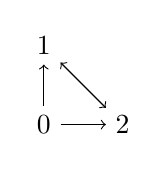
\begin{tikzpicture} 
    \node[] (0) at (0,0) {$0$};
    \node[] (1) at (0,1) {$1$};
    \node[] (2) at (1,0) {$2$};
    \draw[->] (0) -- (2);
    \draw[<->] (1) -- (2);
    \draw[->] (0) -- (1);
  \end{tikzpicture}
  \caption{Graph Test}
  \label{plot:Graph-Test}
\end{figure}

\end{document}

